\documentclass[11pt,a4paper]{article}
\usepackage[utf8]{inputenc}
\usepackage{amsmath}
\usepackage{mathtools}
\usepackage{amsfonts}
\usepackage{amssymb}
\usepackage{graphicx}
\usepackage{caption}
\usepackage{subcaption}
\usepackage{comment}
\usepackage{color}
\usepackage{enumitem}
\usepackage[left=2cm,right=2cm,top=2cm,bottom=2cm]{geometry}
\usepackage{listings}
\usepackage{color}

\setlength{\jot}{10pt}
 
\definecolor{codegreen}{rgb}{0,0.6,0}
\definecolor{codegray}{rgb}{0.5,0.5,0.5}
\definecolor{codepurple}{rgb}{0.58,0,0.82}
\definecolor{backcolour}{rgb}{0.95,0.95,0.92}
 
\lstdefinestyle{mystyle}{
    backgroundcolor=\color{backcolour},   
    commentstyle=\color{codegreen},
    keywordstyle=\color{magenta},
    numberstyle=\tiny\color{codegray},
    stringstyle=\color{codepurple},
    basicstyle=\footnotesize,
    breakatwhitespace=false,         
    breaklines=true,                 
    captionpos=b,                    
    keepspaces=true,                 
    numbers=left,                    
    numbersep=5pt,                  
    showspaces=false,                
    showstringspaces=false,
    showtabs=false,                  
    tabsize=2
}
 
\lstset{style=mystyle}
\graphicspath{ {./figures/} }
\author{Andrew Teta}
\title{ECEN 4532 - Lab 6: Machine Learning}
\date{May 1, 2019}

\begin{document}

\maketitle

\begin{figure}[ht]
	\centering
	
\includegraphics[width=\textwidth]{ml}
\end{figure}

\pagebreak

\tableofcontents

\pagebreak

\section{Introduction}
Researchers in many different fields often collect large quantities of data, with the hope of finding it useful to develop predictions of various phenomena. One very common example in today's age would be advertisement targeting. As users browse the web, certain details about the demographic of people viewing and purchasing products can be collected and stored as a large data set. Machine learning may be a good way to predict what a random user will purchase based on their purchase history or demographic relationship. Many other problems similar to this can be solved using tools like machine learning. Often, they are problems of classification. By classifying users based on their gender, age, region of residency, or other factors, a program or algorithm can predict an outcome for a given activity. The classification involved may be binary or higher order, where a statistic could fall into one of many classification "bins". Other problems may involve continuous predictions. 

When discussing the concept of machine learning, it is helpful to have some motivation and notation. Considering the first example of this lab, we have a domain of objects (passengers on the Titanic) which we would like to classify into categories ("survived or "perished"). Often, the objects are too complex to classify directly and so instead, an array of characteristics for each object are defined as \textit{features}. These features are grouped into a \textit{feature vector}. Each feature vector is referred to as an \textit{instance} and the set of all feature vectors, the \textit{instance space}. 

We will then take a "training set" of data, which correctly maps the instances to its classification. The training set is incomplete and only contains a sample of all the possible instances, so doing our best, we can "learn" an approximation to the real function mapping features to classifications. 

In this lab, we will investigate binary classification using Support Vector Machines, linear regression for predicting a continuous quantity, and multi-class classification using neural networks. The approach here is in the context of data analysis.

\section{Background}
Three data sets will be used for three different classification techniques, respectively. Specifically, we consider:

\begin{itemize}
\item Support Vector Machine (SVM) to predict who survived the sinking of the Titanic. This is an example of a binary classification problem (i.e. "survived" or "perished").
\item Linear regression to predict the water resistance of a sailing yacht based on a selection of design parameters. The predicted value will be a real number here, so this is an example of a continuous classification problem.
\item Neural networking to recognize hand-written digits. This is a multi-class classification problem as there are 10 classes or "bins".
\end{itemize}

For all cases, we will utilize a set of labeled outcomes. As an example, for hand-written digit recognition, we have 70,000 images of numerals 0 through 9, correctly labeled. Thus, we are practicing "supervised" machine learning by fitting an appropriate function to a data set based on a large number of input/output pairs.

\subsection{Support Vector Machines}
A Support Vector Machine (SVM) is a method of binary classification through supervised learning. A model is built based on a training set which can assign a new data point to one classification or the other. It is easiest to understand the process and goal of fitting this model with a graphical representation. Figure \ref{fig:svm} shows that an SVM aims to find the optimal "line", called a \textit{hyperplane} between data points falling into either classification. 

\begin{figure}[ht]
\centering
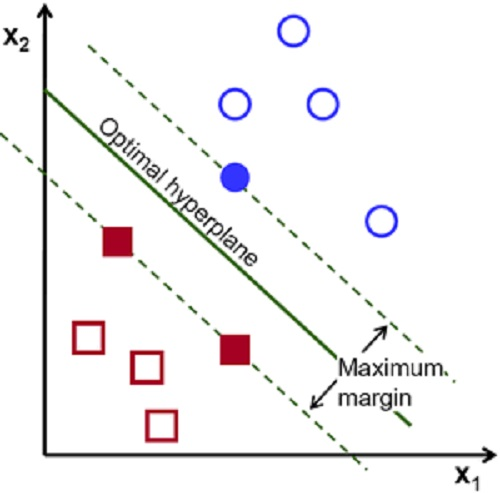
\includegraphics[width=0.4\textwidth]{svm}
\caption{Graphical representation of an SVM hyperplane. \\Credit: https://www.aitrends.com/ai-insider/support-vector-machines-svm-ai-self-driving-cars/}
\label{fig:svm}
\end{figure}

Calling the hyperplane a "line" is inaccurate because really it forms a plane of separation between the feature vectors, represented by red squares and blue circles in fig. \ref{fig:svm}. This plane lives in multidimensional space. If each support vector has dimension $p$, then the hyperplane is of dimension $p-1$. 

As the graphic suggests, another characteristic of SVMs is the margin of the hyperplane. An optimal hyperplane will maximize the margin, effectively finding the largest separation between classifications. Thus, a new data point will fall more decisively on one side of the hyperplane. Furthermore, the vectors defining the margin are called support vectors.

\subsection{Linear Regression}
Fundamentally, the problem of linear regression seeks to find a "best fit" line passing through a data set, to find a model to which predicted data can be fit. The concept of multiple linear regression deals with more than one independent variable. Linear regression is useful when a data set is "over-determined"--often occurring in scientific or statistical measurement. This would be the case where a solution is desired for only one or two dependent variables, but hundreds or thousands of independent variable samples are collected. Then, rather than a single solution to what has become a linear algebra problem, we now have multiple solutions. Through the following proof, we can show that the "best" solution can be found.
We begin with the assumption that we have a set of $N$ measurements, $x_i$, collected together into a vector,

\begin{align*}
\vec{x} = (x_1, x_2, \ldots, x_N)
\end{align*}

Recall, the length of $\vec{x}^2$ is its "energy". Additionally, we will refer to a vector of constants, all equal to $\mu$ as $\vec{\mu}$.
Then, we can define the average energy per vector component of $\vec{x}$ as the error power and call this the \textit{variance}

\begin{align*}
\sigma^2 = \frac{1}{N} |\vec{x} = \vec{\mu}|^2
\end{align*}

where the vertical bars imply vector length and $\vec{\mu}$ is the mean vector of $\vec{x}$.
Finding \textit{standard deviation}, $\sigma$, we have:

\begin{align*}
\sigma = \frac{1}{\sqrt{N}} |\vec{x} - \vec{\mu}|
\end{align*}

Now, considering the case of data point vectors, $\vec{x}$ and $\vec{y}$ (independent/independent variable pairs) we can begin to find a linear regression.
First, we remap each vector into unit vector form:

\begin{align*}
\vec{w} &= \frac{1}{\sigma_x}(\vec{x} - \vec{\mu_x}) \\
\vec{z} &= \frac{1}{\sigma_y}(\vec{y} - \vec{\mu_y})
\end{align*}

We now seek a line, defined by the scalar constants $a$ and $b$, which minimizes the cost (or error power) and write:

\begin{align*}
C(a,b) = |\vec{z} - (a\vec{w} + \vec{b})|^2
\end{align*}

which can be written as a dot product:

\begin{align*}
C(a,b) &= (\vec{z} = (a\vec{w} + \vec{b})) \cdot (\vec{z} - (a\vec{w} + \vec{b})) \\
&= N - 2a\vec{w} \cdot \vec{z} + a^2 N + Nb^2.
\end{align*}

Then, it is possible to show that $N - 2a\vec{w} \cdot \vec{z} + a^2 N$ is a parabola in terms of $a$ and has its minimum at

\begin{align*}
a &= \frac{\vec{w}\vec{z}}{N} \\
&= \frac{\vec{w}}{\sqrt{N}} \cdot \frac{\vec{z}}{\sqrt{N}} \\
&= cos\theta
\end{align*}

Thus, the value $a$ is the correlation coefficient and is the cosine of the angle between the vectors $\vec{w}$ and $\vec{z}$. For notation consistency with other documentation, we will redefine $a= \rho$ and substitute to arrive at:

\begin{align*}
y = \beta x + (\mu_x - \beta \mu_x), \quad	&\text{where $\beta = \rho \frac{\sigma_y}{\sigma_x}$}
\end{align*}

\subsection{Neural Networks}
The basic building blocks of a neural network are "perceptrons" (fig. \ref{fig:nn}) which compute the dot product of its input vector $\vec{x}$, with its weights, $\vec{w}$. The result is passed through a threshold with respect to a bias, $b$ (fig. \ref{fig:nn1}).

\begin{figure}[ht]
\centering
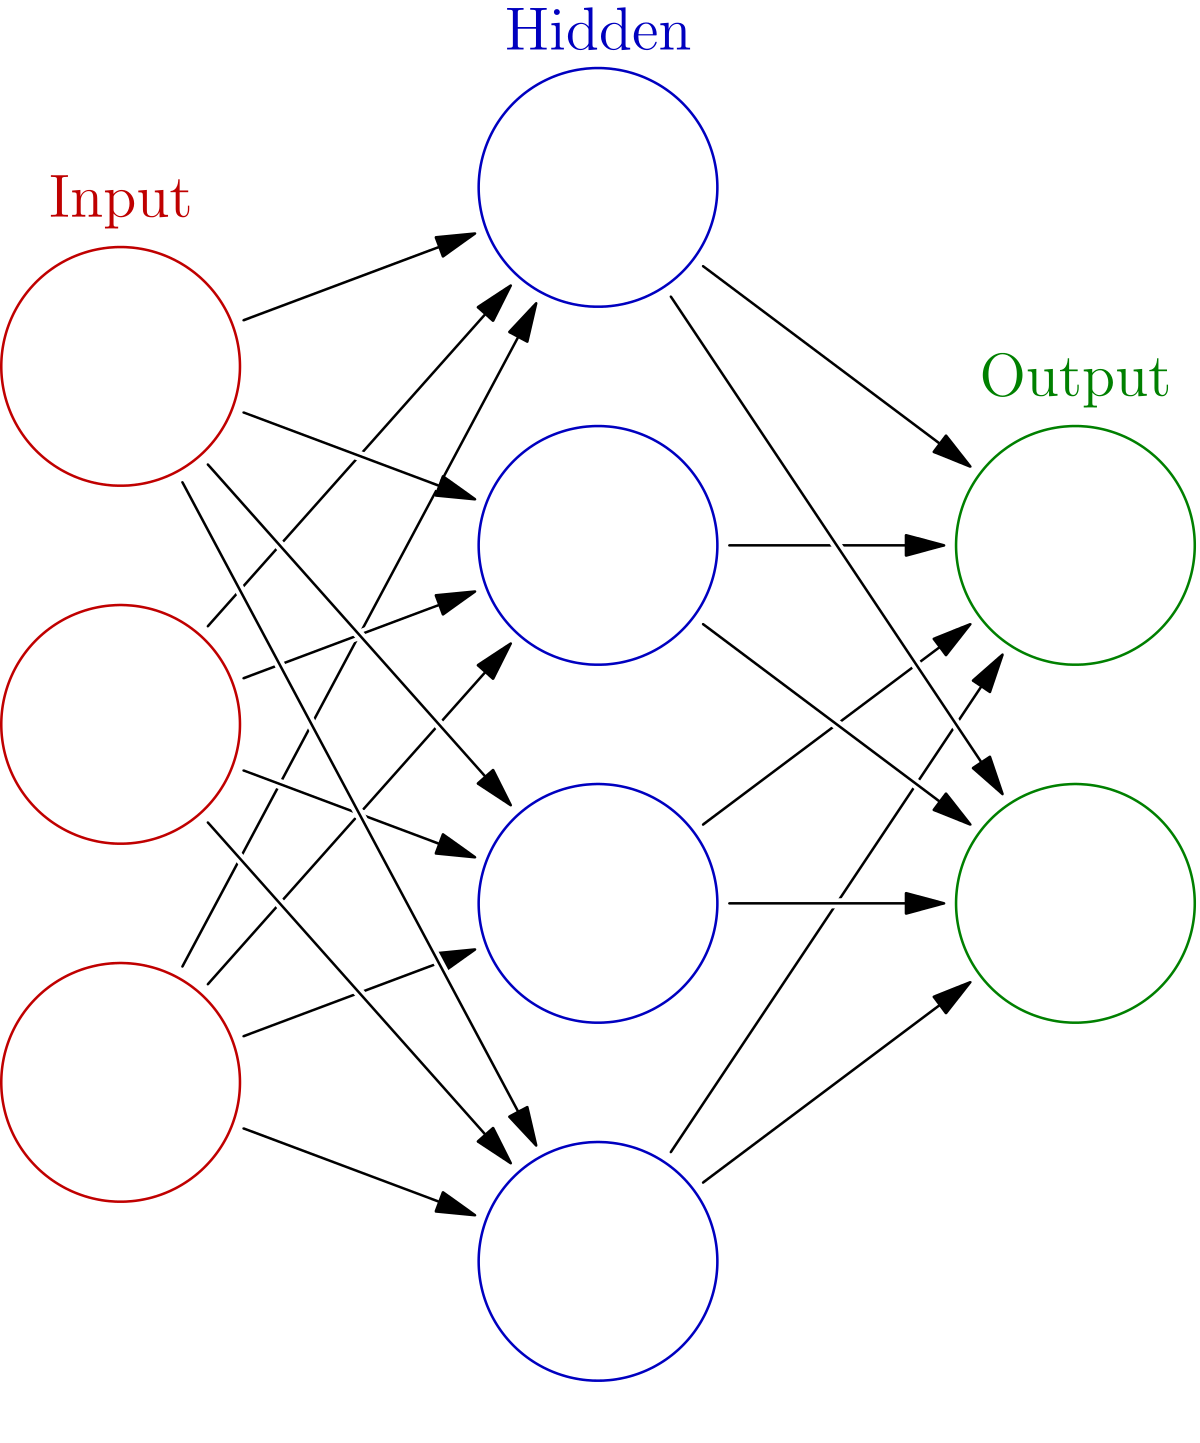
\includegraphics[width=0.4\textwidth]{nn}
\caption{Perceptrons shown on the left.}
\label{fig:nn}
\end{figure}

\begin{figure}[ht]
\centering
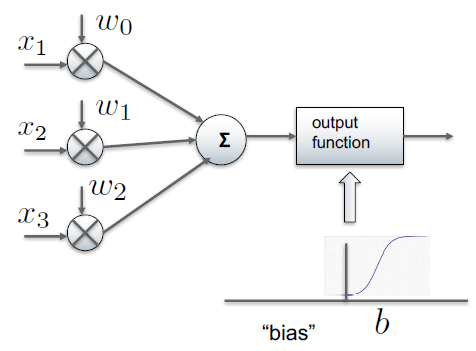
\includegraphics[width=0.6\textwidth]{nn1}
\caption{Inside of a perceptron.}
\label{fig:nn1}
\end{figure}

The process of training a neural network optimizes the parameters of the perceptrons in the network. The hidden layers shown in figure \ref{fig:nn} can be many layers deep and define the complexity of the network, but eventually narrow the input into a single classification at the output layer.

\end{document}